\chapter{Conclusions}

Only a few months might not sound much but is enough to obtain some
conclusion about techonologíes, patterns and ways to develop.
\intro
This work can not finish without a reflexion about what have been the mainly
drawbacks and locks in the develop, design and evolution of the entire project,
trying to propose solutions and overall, learning a lot about all.

\subsection{Scheduling}

The scheduling of development is very easy to do, in the hypothetical case that
all goes fine, but as is normal, there are a lot of factors hard to control that
besides are unknown at the beginning.
\intro
If we join this with an inexpert scrum master and technologies absolutely new for
the team (without a good spikes issues to select and try these) the result can
be catastrophic.
\intro
If we remember the planification that we did in the chapter three, we had estimated
the project in 6 months, that was equeal to 12 sprints, and when them finished
the project would be finished, as can see in the graphic.

\begin{figure}[H]
  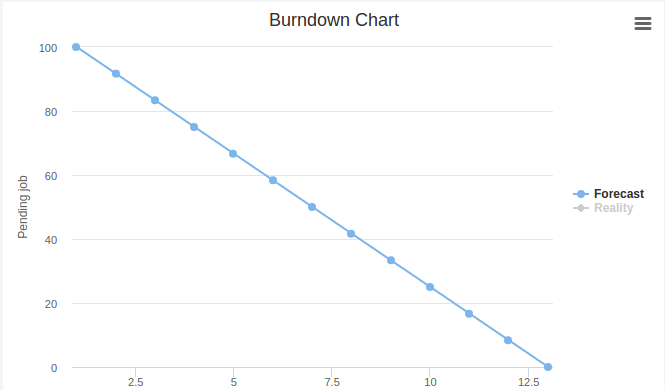
\includegraphics[scale=0.45]{img/graphics/burndown.png}
  \centering
  \caption{Project forecast.}
\end{figure}

\noindent The problem is that the develop has not passed as we would have liked,
and, without going into too much detail, after of our auto evaluation and
evaluation of the sprints and the work that has been finished we can say that
only is finished approximately of 50\% that we expeted to be a stable first version
that we can put in production.
You can see the values in the next graphic.

\begin{figure}[H]
  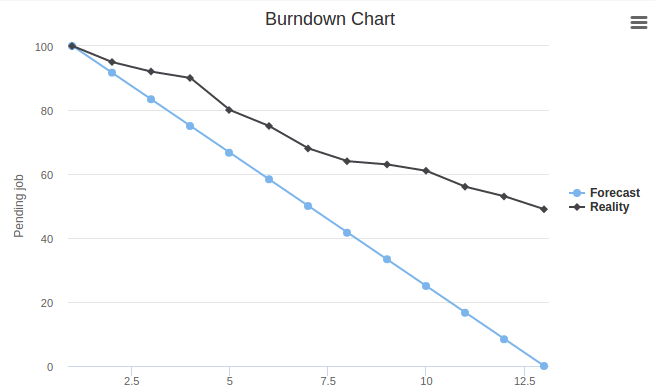
\includegraphics[scale=0.45]{img/graphics/burndown2.png}
  \centering
  \caption{Project forecast and reality.}
\end{figure}

\noindent Obviously, if the project continues, it would need a lot of
modifications and analysis to detect fine-grained which are the reasons
of the 50\% of delay, in addition to those already detected here,
because doing an estimate of the time that at this rithm the project would required
without any modification in the process of production we have that we would need
around 25 sprints, that means another 6 month of develop.

\begin{figure}[H]
  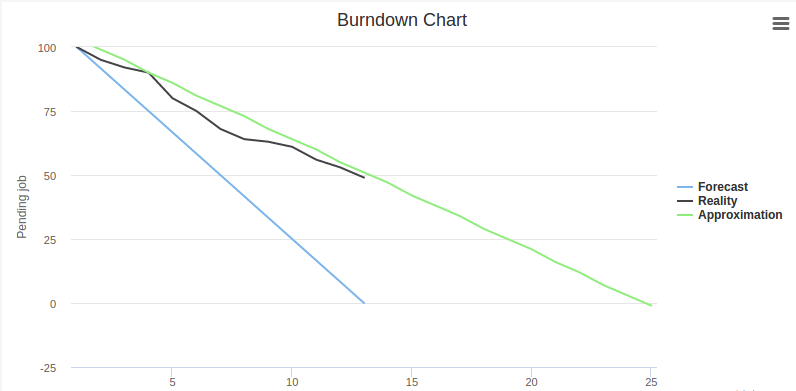
\includegraphics[scale=0.45]{img/graphics/burndown3.png}
  \centering
  \caption{Burndown chart with plannig, workd done and prevision to deadline}
\end{figure}

\noindent These are not good news, the double of time means the double of resources (time and
money) and loose customer confidence, some that we never can not lose.
Despite this, for our feeling, and talking about an pseudo academic work,
the result is not as wrong as could be, and with all predictable fails,
it has not been a bad finish. Knowing that this kind of things only can happens
one time, and should be use to lear and to avoid to make the same mistakes.
\intro
And if we should be do the same project again, our provision would be other
very different, planning exactly the same issues, we calculate that could be
that in less of a half of time, as this forecast shows.

\begin{figure}[H]
  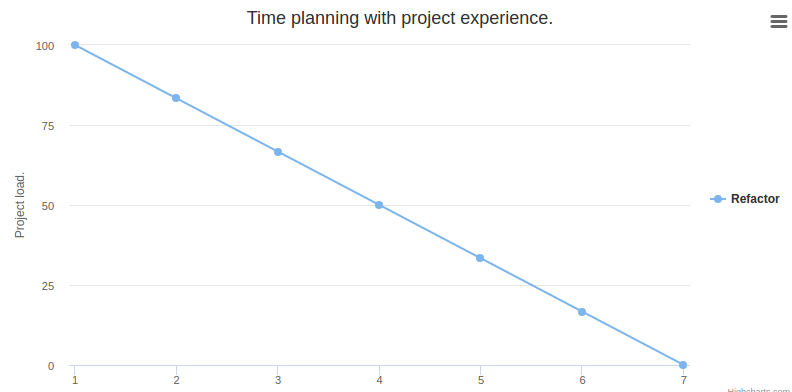
\includegraphics[scale=0.4]{img/graphics/redo.png}
  \centering
  \caption{Replaning experience based.}
\end{figure}

\subsection{Technologies and frameworks}

Of one side, we have the difficulties with the technology choice. In this case
can be said that use AngularJS and Python has been literally perfect, beyond
that the typical novice errors with the languages and their learning curves.
So, in general, without a doubt, they will be chosen as technologies again.
\intro
About the platforms or technologies the point of view changes. If you are
an expert developer using platforms like Google App Engine can be really
interesting, because you are evaluated the rest of the options, but when
you don't have any practice, in my view, is not a good option. Moreover when
the learning curve is so soft.
\intro
As in many new technologies is easy to do the first steps, but develop some bigger
is another thing, especially when we are not talking about frameworks and
languages standard as C++, Java or PHP. So, before to select one is really justify
the spike of some of these.
\intro
About the API frameworks, Flask was a good selection, because their ease of use
and lightness does it perfectly. However, when we analyze the performance, there are
other solutions also in python faster. An example of this is Falcon\footnote{Defined as: \textit{"A
very fast, very minimal Python web framework for building microservices, app backends,
and higher-level frameworks"}. More info at: \textit{falconframework.org}}. As can be
seen in the next picture, extracted from py-frameworks-bench\footnote{
http://klen.github.io/py-frameworks-bench/} project, we can see how Falcon has
better performance than Flask. In this graphic is measure the response in ms
of encode an object to JSON and return the response.

\begin{figure}[H]
  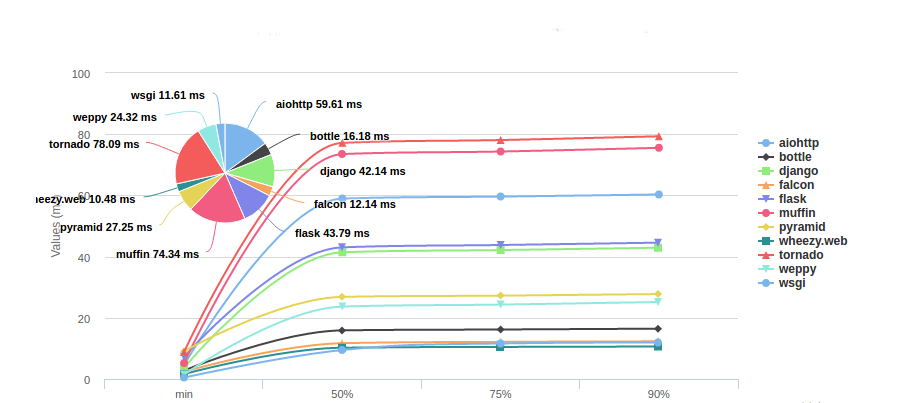
\includegraphics[scale=0.5]{img/graphics/frameworks.png}
  \centering
  \caption{Frameworks performance comparison.}
\end{figure}


\noindent And Falcon would be our selection today (even more having some practice in
company).
\intro
About Sphinx, is a good choice, but it has something that could be improved and
is the requirements of that the project must have. To use Sphinx your project
needs to be \textit{executable}, understanding this as all imports must work.
Many people do not know why Sphinx have this restriction, so if you
only want doc, independently of if you structure is correct or not, well, this is
impossible in the actual version, we hope that change this at any moment.

\subsubsection{About the platform}

In spite of Google App Engine is a good tool it has some drawbacks that some are
very obvious at first and others that can go unnoticed until you are working with it.
the sandbox restrictions as use python only in their version 2.7 at first is not
a problem but when you discover that the most of the libraries that you need works
better in 3.x, or some are deprecated in 2.7, out of maintenance is not a good
signal, especially when you have some block and the help of community is focused
on upper versions. It happened in the standard version of App Engine sandbox, to
solve this the team of it launched App Engine Flexible Environment, where you can
run any code but the configuration is not trivial and it although is configurable by
docker file is a strange mix between the auto maintained and scalable isolated
sandbox and the standard containers developer managed.
\intro
So, taking advantage of all services of the infrastructure of GCE, another
architecture that we will develop in the future will run only into docker containers,
using the services required (SQL, DataStore or another and running over compute layer,
not with google app engine.

\subsubsection{About the database}

About database, without doubt, MongoDB is nowadays the better solution that
can be used in a project with low relational requirements, because their learning
curve is so good that is easy to have a good prototype of database layer soon,
and the resources of the community greatly assist.

\subsection {Design}

\subsubsection{About the user interface}

There are any that has been critical in the develop and is that the assumption
as a good idea that all interface always is loaded when a user enters to the app,
but after some tests have been seen that is not the best way.  For this reason,
many teams that work with Angular choose an alternative, use a library specially
designed to load the javascript files of the app needed in each part of the interface.
\intro
So, if a user is in the teaching section don't need all files of the reports section, and this files only will be loaded when the user insert in this section. To do this,
the teams use the Require.js\footnote{Literraly from their website ,requirejs.org: \textit{"RequireJS is a
JavaScript file and module loader. It will improve the speed and quality of your code."}} library as
the standard dynamically loader and their use will be the next step to do the
load of the app faster.
\subsubsection{About the compression of APIs}

Is easy to notice that the API of Students Control microService is very semantic
but very big also (become more complex to maintain and change) while of the
teaching service API is very compact and little but less semantic, because the
meaning of their resources is not clear and therefore their behavior neither.
It was made on purpose it to check in the development which approach was more
problematic or simple to explain or update.
\intro
And the conclusion is that to maintain the coherency between the domain drive
development of the service and the expressivity of the API the customers do not
need to know the internal work of the service, but need understand the logic
behind of the items, so, in the future, it will be moved to an approach more human
readable (in spite of all disadvantages, talking about code and maintenance).

\subsection{The develop process}

Can be really interesting if you use any methodology as SCRUM and the developer's
team work together. But when the team is a single developer and the project only
have sporadic contributions,
all is more difficult to follow. Other techniques can be used but SCRUM, eXPrograming
or something like this not works fine to only one person.
\intro
So, independently, is a good point to start to practice. On other hand, is
noticed that the sporadic contributions as in a hackathon\footnote{Is an event based on a sprint
in which computer programmers and others are involved in the development of some software} or
in a simple day are difficult too because, as is normal, the people require a time to understand the
project, the technology and all related with it.
\intro
As we comment before if we does not have a good overview of the project to long-term
and we not foresee the growth of it, we can get a point where the code is too big
or messy that to require a big refactoring.
This would make us lose a lot of time of development (that was not planned) and
even though is better detect this early, it will be a problem.
An example of this was the point of the development where was necessary to do a
refactor. See chart bellow.

\begin{figure}[H]
  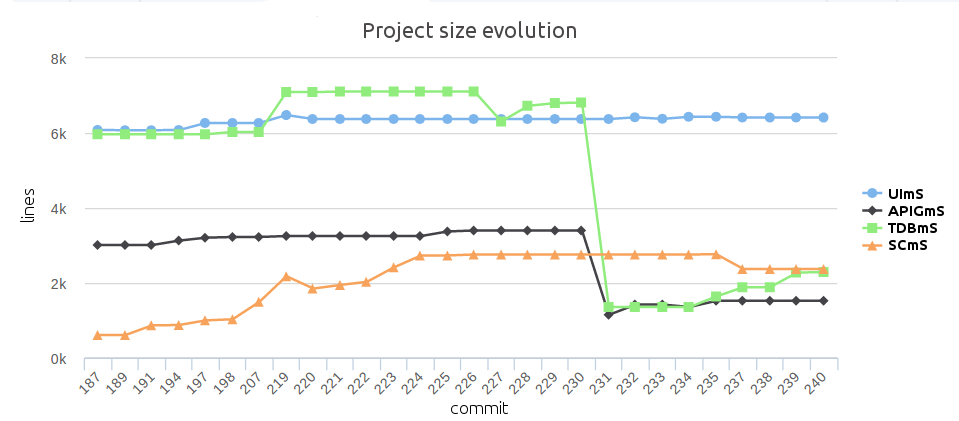
\includegraphics[scale=0.45]{img/graphics/repository_size.png}
  \centering
  \caption{Project size in lines and refactoring effect.}
\end{figure}

\noindent As we can see, we had services that not stop to grow despite the logic
was not very complex. It was because it was used some technologies that after was
discarded. And after, the weight of the services was reduced drastically (the rest
of services was a normal grow), to something more normal, having less code to
maintain, cleaning and documenting, doing a lot more of things that before the
refactoring. We would like to remind a great book about refactoring, \cite{refactor}).


\subsection{Opportunities}

Take part of some software contest is the better decision that any
software student can take. Visibility, networking, new friendship are only some
benefits that can achieve.
\intro
Thanks to enrolling this project of the contests that the Open Source Department of
the University of Granada with JJ Merelo as principal organizes was offer a job
in a related software company with the technologies and patterns used.
So, if any people think that the participation, the contribution, and involvement
is not useful, is absolutely wrong. In all cases, this attitude front the
students only return benefits.

\subsection{Future of the project}

At the beginning of the develop, the idea behind of this was put in production
the result in a few months in beta mode in a school center of Granada, but now,
the jobs opportunities referred above have been done that the project go to the
another plane, less important, because the ideas and the philosophy are
developed just now with another really good engineers in a company, building a
privative software, architecture, and new related tools.
\intro
So, independently the license of the code has not changed, and the develop can
go ahead with any developer or group of them that want. For another hand the
continuous evolution of the technologies do this issue a
bit difficult, and actually, it is another learned lesson about the innovate
software using three party technologies, we will never have the safety that the
technology never will change. If you are working with C++ or even Java with you
own infrastructure the changes are minimal through the months, with third party
technologies and support you need be at day with all changes and update almost
all your software each year. So, in this cases is difficult that the continuity
of the project will be ensured, at least without the original designer inside the
new developer's teams. But, anyway, is only a point of view, with the software
nothing can be assumed.
\intro
Independently, the code is open, to learn, to review, and maybe to help someone,
so for this part, we are happy.

\subsubsection{Data processing}

Finally the project has not grow as much as we would have liked, and this part
is not enough powerful to their possibilities. The huge amount of data joined
with their clear relations does this especially interesting to apply techniques
as data mining or machine learning. The simple relations between data is easy
to see but can be exists dozen of interesting relations that can go undetected
and their work will be the mainly task in futures iterations.

\subsection{Open Source}

Other conclusions obtained in the solution development are related to open source and the
viability to survive on this. Many time in the college is easy to hear that the
open source is a good way to start and is true, but not if you want to work of
this. Work in open source projects is really interesting, for the community,
for the workflow, for build some useful to the community and by a huge list of
advantages. But this is possible only when for one hand you are working in a
company and some of the projects of this are decided to be open, independently of the
reason, community, better visibility, etc. or when you are a student and have
the opportunity to free amounts of code, as this case. But for another hand,
thinking to build a company, more o less big based on an open source solution
is very very rare and complex, mainly to younger and inexpert software developers.
\intro
Obviously in the most cases, always there are some exceptions that are
wonderful examples that project with an amazing grow, and a really amount of
code that any developer must have would be open, always open, because there
are any developer that can learn alone, without the community (in any of their
forms) and be in the obligation to contribute, to give back the favor.

\subsection{Closing}
This project has been a great opportunity to learn a lot about amount of things,
but especially about myself, has been another opportunity to know how to deal with
new challenges, how to work a first really subtle approach to project management and
the most important, to know which my bigger faults.
It have helped me to understand that this is only the begin, the beginning of
the way that only can be covered if you do not stop to learn never, absolutely never.
\intro
So, \textbf{let's start!}
